\documentclass[11pt,a4paper]{article}

\usepackage[utf8]{inputenc}
\usepackage[T1]{fontenc}
\usepackage{lmodern}
\usepackage[margin=2.5cm]{geometry}
\usepackage{graphicx}
\usepackage{xcolor}
\usepackage{listings}
\usepackage{booktabs}
\usepackage{array}
\usepackage{tabularx}
\usepackage{caption}
\usepackage{float}
\usepackage{enumitem}
\usepackage{hyperref}
\usepackage{tikz}
\usetikzlibrary{positioning,arrows.meta,calc,shapes.geometric}

\hypersetup{
  colorlinks=true,
  linkcolor=black,
  urlcolor=blue!50!black,
  pdftitle={Cipher-16: A 16-bit Cryptographic Coprocessor in VHDL}
}

% VHDL listing style
\definecolor{kwblue}{RGB}{0,90,170}
\definecolor{cmtgray}{RGB}{110,110,110}
\definecolor{strred}{RGB}{160,40,40}
\definecolor{bgshade}{RGB}{248,248,248}

\lstdefinelanguage{VHDL}{
  morekeywords={
    library,use,entity,is,port,in,out,end,architecture,of,begin,
    process,if,then,elsif,else,case,when,others,signal,std_logic,
    std_logic_vector,downto,to,rising_edge,with,select,map,work,
    array,type,not,and,or,xor,unsigned,integer,natural,constant,
    procedure,wait,assert,report,severity,generic
  },
  sensitive=false,
  morecomment=[l]{--},
  morestring=[b]"
}

\lstset{
  language=VHDL,
  basicstyle=\ttfamily\footnotesize,
  keywordstyle=\color{kwblue}\bfseries,
  commentstyle=\color{cmtgray}\itshape,
  stringstyle=\color{strred},
  backgroundcolor=\color{bgshade},
  frame=single,
  rulecolor=\color{black!20},
  numbers=left,
  numberstyle=\tiny\color{black!50},
  numbersep=8pt,
  showstringspaces=false,
  breaklines=true,
  captionpos=b,
  tabsize=2,
  xleftmargin=1em
}

\begin{document}

% =====================================================================
% COVER PAGE
% =====================================================================
\begin{titlepage}
  \centering
  \vspace*{1cm}

  {\scshape\Large Zagazig University \par}
  {\scshape\large Faculty of Engineering \par}
  {\scshape\large Computer and Systems Engineering Department \par}
  \vspace{0.4cm}
  {\large CSE 226: Hardware Design \par}

  \vspace{2.5cm}
  \rule{\linewidth}{0.5pt}\par
  \vspace{0.8cm}
  {\huge\bfseries Cipher-16 \par}
  \vspace{0.4cm}
  {\Large A 16-bit Cryptographic Coprocessor in VHDL \par}
  \vspace{0.6cm}
  \rule{\linewidth}{0.5pt}\par

  \vspace{1.5cm}
  {\large\itshape Project Report \par}
  \vspace{0.3cm}
  {\large Submitted: \today \par}

  \vspace{1.5cm}

  {\large\bfseries Team Members \par}
  \vspace{0.4cm}
  \begin{tabular}{c}
    Mohamed Emad ElSawy \\[2pt]
    Mohamed Mahmoud Ramadan \\[2pt]
    Mohamed Ali Mohamed \\[2pt]
    Mohamed Magdy Hendawy \\[2pt]
    Mohamed Mustafa ElSayed \\
  \end{tabular}

  \vfill

  \begin{tabular}{rl}
    \textbf{Course} & CSE 226: Hardware Design \\
    \textbf{Tools}  & GHDL, GTKWave, Active-HDL \\
    \textbf{HDL}    & VHDL (IEEE 1076) \\
  \end{tabular}

  \vspace{1cm}
\end{titlepage}

% =====================================================================
% TABLE OF CONTENTS
% =====================================================================
\tableofcontents
\newpage

% =====================================================================
% 1. ASSIGNMENT AIM
% =====================================================================
\section{The Assignment Aim}

The assignment is to design and verify a 16-bit cryptographic
coprocessor in VHDL. The coprocessor is the datapath of a small
hardware accelerator that performs the inner operations used by block
ciphers: register-to-register reads, non-linear substitution through
S-Boxes, arithmetic and logical operations through an ALU, and
bit-level rotations through a shifter.

The work covers the full RTL flow:
\begin{itemize}[leftmargin=*]
  \item Partition the design into reusable components (register file,
        non-linear lookup unit, shifter, ALU, combinational block,
        top-level coprocessor).
  \item Define a single 4-bit \texttt{CTRL} encoding that selects
        between the functional units.
  \item Wire the components together inside a clocked top-level entity
        with an asynchronous reset and an input register that stages
        the operand and opcode fields.
  \item Verify each block with its own testbench, then verify the
        integrated coprocessor with a self-checking testbench that
        exercises reset, LUT substitution, write-back, the ALU path,
        the shifter path, and reset-while-running behaviour.
\end{itemize}

The deliverables are the synthesisable VHDL source for each block, a
schematic of the top-level entity captured in Active-HDL, simulation
waveforms produced by GHDL/GTKWave, and this report.

% =====================================================================
% 2. PROBLEM SOLUTION
% =====================================================================
\section{The Problem Solution}

The coprocessor is organised as two cooperating blocks:

\begin{enumerate}[leftmargin=*]
  \item A \textbf{datapath} consisting of a 16$\times$16 register file
        preceded by an input pipeline register. The input register
        captures \texttt{Ra}, \texttt{Rb}, \texttt{Rd} and
        \texttt{CTRL} on the rising clock edge; the register file
        exposes the two operand registers on \texttt{A\_BUS} and
        \texttt{B\_BUS}, and writes the previous-cycle result back to
        \texttt{R[Rd]}.
  \item A \textbf{combinational logic block} that drives the result
        bus from one of three functional units (a non-linear
        lookup operation unit with two S-Boxes, an ALU, and a
        shifter), under control of a small decoder that interprets
        \texttt{CTRL}.
\end{enumerate}

The functional unit driving \texttt{RESULT} is chosen by the decoder
according to Table \ref{tab:ctrl-routing}.

\begin{table}[H]
  \centering
  \caption{CTRL routing in the combinational block.}
  \label{tab:ctrl-routing}
  \begin{tabular}{@{}lll@{}}
    \toprule
    \textbf{CTRL[3]} & \textbf{CTRL[1:0]} & \textbf{Selected unit} \\
    \midrule
    0 & --     & Non-Linear Lookup (S-Boxes) \\
    1 & 11     & Shifter                     \\
    1 & other  & ALU                         \\
    \bottomrule
  \end{tabular}
\end{table}

The shifter recognises three opcodes; any other code drives a zero
output (Table \ref{tab:shifter-ops}).

\begin{table}[H]
  \centering
  \caption{Shifter opcodes.}
  \label{tab:shifter-ops}
  \begin{tabular}{@{}lll@{}}
    \toprule
    \textbf{CTRL} & \textbf{Operation} & \textbf{Effect on B\_BUS} \\
    \midrule
    1000  & ROR8 & 8-bit right rotation \\
    1001  & ROR4 & 4-bit right rotation \\
    1010  & SLL8 & 8-bit left shift, zero-filled \\
    other & (none) & SHIFT\_OUT = 0x0000 \\
    \bottomrule
  \end{tabular}
\end{table}

The non-linear lookup unit splits the low 8 bits of \texttt{A\_BUS}
into two 4-bit halves: the lower half is mapped through S-Box~1, the
upper half through S-Box~2 (Table \ref{tab:sboxes}). The two 4-bit
outputs are concatenated and merged with the unchanged high byte of
\texttt{A\_BUS} to produce the 16-bit result.

\begin{table}[H]
  \centering
  \caption{S-Box substitution tables (4-bit $\to$ 4-bit).}
  \label{tab:sboxes}
  \small
  \begin{tabular}{@{}cc@{\hspace{1.2cm}}cc@{}}
    \toprule
    \multicolumn{2}{c}{\textbf{S-Box 1}} & \multicolumn{2}{c}{\textbf{S-Box 2}} \\
    Input & Output & Input & Output \\
    \midrule
    0000 & 0001 & 0000 & 1111 \\
    0001 & 1011 & 0001 & 0000 \\
    0010 & 1001 & 0010 & 1101 \\
    0011 & 1100 & 0011 & 0111 \\
    0100 & 1101 & 0100 & 1011 \\
    0101 & 0110 & 0101 & 1110 \\
    0110 & 1111 & 0110 & 0101 \\
    0111 & 0011 & 0111 & 1010 \\
    1000 & 1110 & 1000 & 1001 \\
    1001 & 1000 & 1001 & 0010 \\
    1010 & 0111 & 1010 & 1100 \\
    1011 & 0100 & 1011 & 0001 \\
    1100 & 1010 & 1100 & 0011 \\
    1101 & 0010 & 1101 & 0100 \\
    1110 & 0101 & 1110 & 1000 \\
    1111 & 0000 & 1111 & 0110 \\
    \bottomrule
  \end{tabular}
\end{table}

\subsection{Inputs and Outputs}

The top-level entity \texttt{coprocessor} exposes a register-mapped
control interface; all data resides in the internal register file and
is read or written through register indices.

\begin{table}[H]
  \centering
  \caption{Coprocessor port list.}
  \label{tab:ports}
  \renewcommand{\arraystretch}{1.15}
  \begin{tabularx}{\linewidth}{@{}l l l X@{}}
    \toprule
    \textbf{Port} & \textbf{Dir} & \textbf{Width} & \textbf{Function} \\
    \midrule
    \texttt{clock}  & in  & 1  & System clock. All sequential elements update on the rising edge. \\
    \texttt{reset}  & in  & 1  & Asynchronous, active-high. Clears the input register and zeroes every register-file location. \\
    \texttt{CTRL}   & in  & 4  & Opcode. Selects the functional unit and (for ALU/Shifter) the operation. \\
    \texttt{Ra}     & in  & 4  & Index of the source-A register. Drives \texttt{A\_BUS}. \\
    \texttt{Rb}     & in  & 4  & Index of the source-B register. Drives \texttt{B\_BUS}. \\
    \texttt{Rd}     & in  & 4  & Index of the destination register. Receives the previous-cycle \texttt{RESULT}. \\
    \texttt{RESULT} & out & 16 & Combinational output of the selected functional unit for the current operands. \\
    \bottomrule
  \end{tabularx}
\end{table}

\noindent\textbf{Internal buses.} \texttt{A\_BUS} and \texttt{B\_BUS}
are 16-bit signals between the register file and the combinational
block; they are not exposed at the top-level ports. The non-linear
lookup unit only consumes \texttt{A\_BUS[7:0]}; the upper byte is
forwarded unchanged.

\noindent\textbf{Pipeline behaviour.} Because the operand fields pass
through the input register, an instruction issued on edge $N$ produces
its \texttt{RESULT} during cycle $N$ and is written back to
\texttt{R[Rd]} on edge $N+1$. A read of a register that was the
destination of the previous instruction therefore returns the value
written one cycle earlier.

% =====================================================================
% 3. IMPLEMENTATION
% =====================================================================
\section{Implementation}

The design is split across five VHDL files in \texttt{src/}, each
defining one entity. The top-level \texttt{coprocessor} entity
instantiates the register file and the combinational block; the
combinational block in turn instantiates the lookup unit, the ALU and
the shifter.

\subsection{Source Modules}

\begin{table}[H]
  \centering
  \caption{Source files and the entities they define.}
  \begin{tabularx}{\linewidth}{@{}l X@{}}
    \toprule
    \textbf{File} & \textbf{Role} \\
    \midrule
    \texttt{coprocessor.vhd}         & Top entity. Input register + register file + combinational block. \\
    \texttt{register\_file.vhd}      & 16$\times$16 register array. Combinational reads, synchronous write. \\
    \texttt{combinational\_circuit.vhd} & Functional-unit MUX driven by the \texttt{CTRL} decoder. \\
    \texttt{non\_linear\_lookup.vhd} & Two-S-Box substitution on the low byte of \texttt{A\_BUS}. \\
    \texttt{shifter.vhd}             & Rotation/shift unit driven by \texttt{CTRL}. \\
    \texttt{alu.vhd}                 & Arithmetic Logic Unit. \\
    \bottomrule
  \end{tabularx}
\end{table}

\noindent The top entity stages every input through a clocked register
before driving the rest of the datapath. This guarantees that the
operand indices and the opcode are stable for a full cycle while the
combinational block settles.

\begin{lstlisting}[caption={Top-level entity (\texttt{src/coprocessor.vhd}, abridged).}]
entity coprocessor is
  port (
    clock  : in  std_logic;
    reset  : in  std_logic;
    CTRL   : in  std_logic_vector(3 downto 0);
    Ra     : in  std_logic_vector(3 downto 0);
    Rb     : in  std_logic_vector(3 downto 0);
    Rd     : in  std_logic_vector(3 downto 0);
    RESULT : out std_logic_vector(15 downto 0)
  );
end coprocessor;

architecture rtl of coprocessor is
  signal Ra_reg, Rb_reg, Rd_reg, CTRL_reg : std_logic_vector(3 downto 0);
  signal A_BUS, B_BUS, result_s           : std_logic_vector(15 downto 0);
begin
  input_reg: process(clock, reset)
  begin
    if reset = '1' then
      Ra_reg <= (others => '0'); Rb_reg <= (others => '0');
      Rd_reg <= (others => '0'); CTRL_reg <= (others => '0');
    elsif rising_edge(clock) then
      Ra_reg <= Ra; Rb_reg <= Rb; Rd_reg <= Rd; CTRL_reg <= CTRL;
    end if;
  end process;

  reg_file: entity work.register_file port map (
    clk=>clock, rst=>reset, RdWEn=>'1',
    Ra=>Ra_reg, Rb=>Rb_reg, Rd=>Rd_reg,
    Res=>result_s, SRCa=>A_BUS, SRCb=>B_BUS);

  comb_logic: entity work.combinational_circuit port map (
    ABUS=>A_BUS, BBUS=>B_BUS, CTRL=>CTRL_reg, Result=>result_s);

  RESULT <= result_s;
end architecture;
\end{lstlisting}

\noindent The decoder inside \texttt{combinational\_circuit} matches
the routing rules in Table \ref{tab:ctrl-routing}.

\begin{lstlisting}[caption={CTRL decoder driving the result MUX.}]
control_logic: process(CTRL, tmp_out1, tmp_out2, tmp_out3)
begin
  case CTRL(3) is
    when '0'   => RESULT <= tmp_out1;            -- LUT path
    when others =>
      case CTRL(1 downto 0) is
        when "11"   => RESULT <= tmp_out3;       -- Shifter path
        when others => RESULT <= tmp_out2;       -- ALU path
      end case;
  end case;
end process;
\end{lstlisting}

\subsection{Schematic Diagram (Active-HDL)}
\label{sec:schematic}

The schematics in this subsection are the RTL views exported after
elaborating each entity. Figure~\ref{fig:schematic-top} is the
top-level view that ties the four input registers, the register
file, and the combinational block together; the remaining figures
zoom into each sub-block.

\begin{figure}[H]
  \centering
  \includegraphics[width=\linewidth]{../rtl-views/Top-view.pdf}
  \caption{Top-level coprocessor schematic: input pipeline
  registers, register file, combinational block.}
  \label{fig:schematic-top}
\end{figure}

\begin{figure}[H]
  \centering
  \includegraphics[width=0.95\linewidth,keepaspectratio]{../rtl-views/CLU.pdf}
  \caption{Combinational logic block: ALU, LUT, Shifter, and the
  per-bit result MUX driven by the CTRL decoder.}
  \label{fig:schematic-clu}
\end{figure}

\begin{figure}[H]
  \centering
  \includegraphics[width=\linewidth,keepaspectratio]{../rtl-views/Register.pdf}
  \caption{16$\times$16 register-file RTL view: synchronous write
  port and two combinational read ports.}
  \label{fig:schematic-reg}
\end{figure}

\begin{figure}[H]
  \centering
  \includegraphics[width=\linewidth,keepaspectratio]{../rtl-views/ALU.pdf}
  \caption{ALU RTL view.}
  \label{fig:schematic-alu}
\end{figure}

\begin{figure}[H]
  \centering
  \includegraphics[width=\linewidth,keepaspectratio]{../rtl-views/Shifter.pdf}
  \caption{Shifter RTL view: bit-wise routing for ROR8, ROR4,
  and SLL8.}
  \label{fig:schematic-shifter}
\end{figure}

\begin{figure}[H]
  \centering
  \includegraphics[width=\linewidth,keepaspectratio]{../rtl-views/LUT.pdf}
  \caption{Non-linear lookup (S-Box) RTL view.}
  \label{fig:schematic-lut}
\end{figure}

\subsection{Simulation Results}

The coprocessor is verified by \texttt{tb/coprocessor\_tb.vhd}, a
self-checking testbench that drives the inputs through a sequence of
operations and asserts the expected value of \texttt{RESULT} after
each clock tick. The clock period is 20\,ns; assertions are sampled a
quarter-period after each rising edge so that the combinational path
has fully settled.

\subsubsection*{Test sequence}

\begin{enumerate}[leftmargin=*]
  \item \textbf{Reset.} Hold \texttt{reset = '1'} for two cycles. All
        registers and the input register are zero, so \texttt{CTRL\_reg = 0000}
        routes the path through the LUT.
        \texttt{LUT(0x0000) = sbox2(0) \,\&\, sbox1(0) = 0xF1};
        the high byte of \texttt{A\_BUS} is zero, giving
        \texttt{RESULT = 0x00F1}.
  \item \textbf{LUT read.} Release reset; read \texttt{R[5] = 0} and
        target \texttt{Rd = 10} with \texttt{CTRL = 0000}. Expected:
        \texttt{RESULT = 0x00F1}.
  \item \textbf{Write-back verification.} The next tick writes
        \texttt{0x00F1} into \texttt{R[10]}. Reading \texttt{R[10]}
        with \texttt{CTRL = 0000} routes \texttt{LUTIN = 0xF1} through
        the S-Boxes: \texttt{sbox1(1) = 0xB}, \texttt{sbox2(F) = 0x6},
        so \texttt{RESULT = 0x006B}. Observing this value proves the
        previous-cycle write took effect.
  \item \textbf{ALU path.} \texttt{CTRL = 1000} satisfies
        \texttt{CTRL[3]='1'} and \texttt{CTRL[1:0]="00"}, routing to
        the ALU. The current ALU does not decode opcode \texttt{1000},
        so \texttt{ALUOUT = 0x0000} and the assertion expects
        \texttt{0x0000}.
  \item \textbf{ALU path (subtract opcode).} \texttt{CTRL = 1001}
        likewise routes to the ALU; opcode \texttt{1001} is
        undecoded, so \texttt{RESULT = 0x0000}.
  \item \textbf{Shifter path.} \texttt{CTRL = 1011} selects the
        shifter (\texttt{CTRL[1:0]="11"}). \texttt{1011} is outside
        the shifter's three-opcode table, so the shifter drives
        \texttt{0x0000}.
  \item \textbf{Reset after instructions.} Re-asserting \texttt{reset}
        asynchronously clears all registers; on the next tick the
        path returns to the LUT and \texttt{RESULT} settles back to
        \texttt{0x00F1}.
\end{enumerate}

\subsubsection*{Expected values}

\begin{table}[H]
  \centering
  \caption{Self-checking assertions in \texttt{coprocessor\_tb}.}
  \label{tab:expected}
  \begin{tabular}{@{}llllll@{}}
    \toprule
    \textbf{Step} & \textbf{CTRL} & \textbf{Ra} & \textbf{Rd} & \textbf{Path} & \textbf{Expected RESULT} \\
    \midrule
    Reset                & 0000 & 0    & 0    & LUT     & 0x00F1 \\
    LUT read             & 0000 & 5    & 10   & LUT     & 0x00F1 \\
    Write-back probe     & 0000 & 10   & 9    & LUT     & 0x006B \\
    ALU (op 1000)        & 1000 & 10   & 8    & ALU     & 0x0000 \\
    ALU (op 1001)        & 1001 & 10   & 7    & ALU     & 0x0000 \\
    Shifter (op 1011)    & 1011 & 10   & 6    & Shifter & 0x0000 \\
    Reset after run      & n/a   & n/a  & n/a  & LUT     & 0x00F1 \\
    \bottomrule
  \end{tabular}
\end{table}

\subsubsection*{Running the simulation}

\begin{lstlisting}[language=bash, basicstyle=\ttfamily\footnotesize,
  keywordstyle=\color{kwblue}\bfseries, frame=single,
  backgroundcolor=\color{bgshade}, numbers=none]
$ make coprocessor                # compile and run the testbench
$ make simu                       # open the .vcd files in GTKWave
\end{lstlisting}

\noindent The testbench writes \texttt{simu/coprocessor.vcd}, which is
opened with GTKWave for inspection. All assertions pass, ending with
the message \texttt{All coprocessor tests PASSED}.

Each block has its own VCD captured under GHDL and rendered from the
raw event stream. Figures \ref{fig:wave-nll} through
\ref{fig:wave-cop} follow the same convention: 1-bit signals are
drawn as digital traces, multi-bit buses are drawn as hex-labelled
segments.

\paragraph{Non-linear lookup unit (S-Boxes).}
Figure~\ref{fig:wave-nll} steps \texttt{LUTIN} through a sweep of
input values. Each output is the concatenation
\texttt{sbox2(high) \,\&\, sbox1(low)}.

\begin{figure}[H]
  \centering
  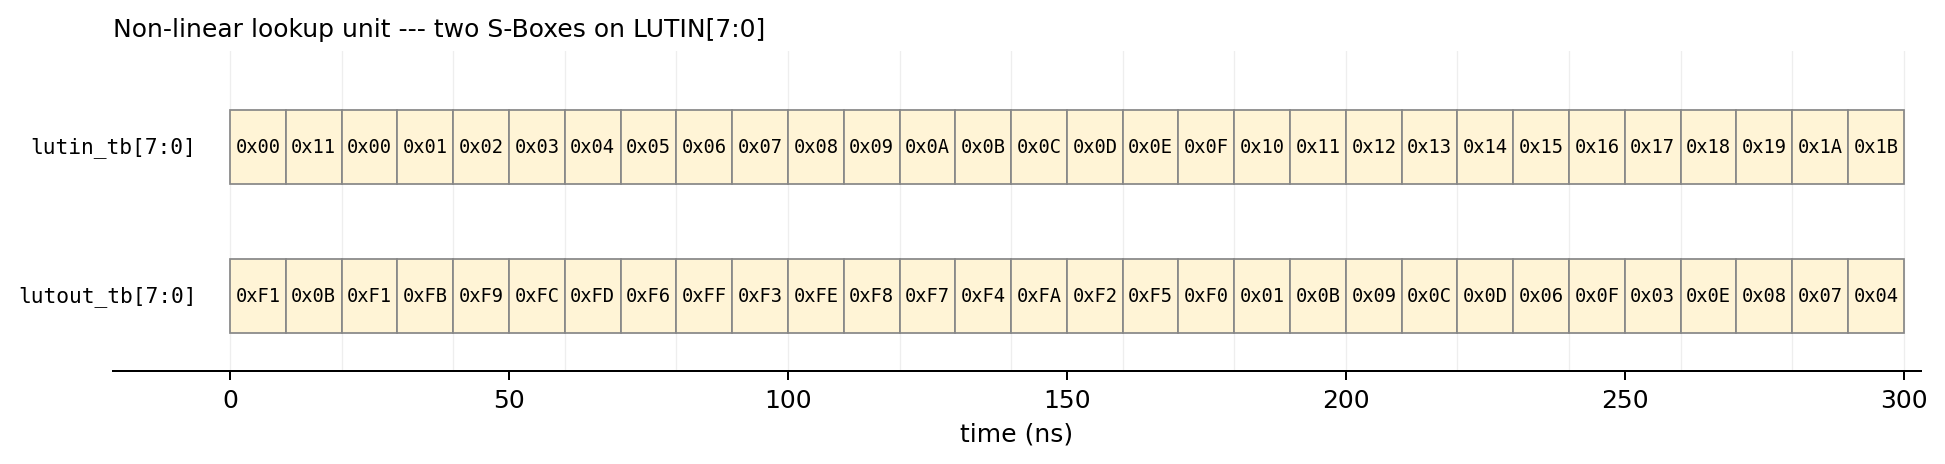
\includegraphics[width=\linewidth]{figures/waveform_non_linear_lookup.png}
  \caption{Non-linear lookup waveform
  (\texttt{report/vcd/non\_linear\_lookup.vcd}).}
  \label{fig:wave-nll}
\end{figure}

Spot checks: \texttt{LUTIN=0x00} $\to$ \texttt{0xF1}
(\texttt{sbox2(0)=F}, \texttt{sbox1(0)=1});
\texttt{LUTIN=0x11} $\to$ \texttt{0x0B}
(\texttt{sbox2(1)=0}, \texttt{sbox1(1)=B});
\texttt{LUTIN=0x1F} $\to$ \texttt{0x00}
(\texttt{sbox2(1)=0}, \texttt{sbox1(F)=0}).

\paragraph{Shifter.}
Figure~\ref{fig:wave-shifter} drives \texttt{b\_in} with two test
patterns (\texttt{0xDEAD} and \texttt{0x1234}) and cycles through the
shifter's three valid opcodes plus one undefined code.

\begin{figure}[H]
  \centering
  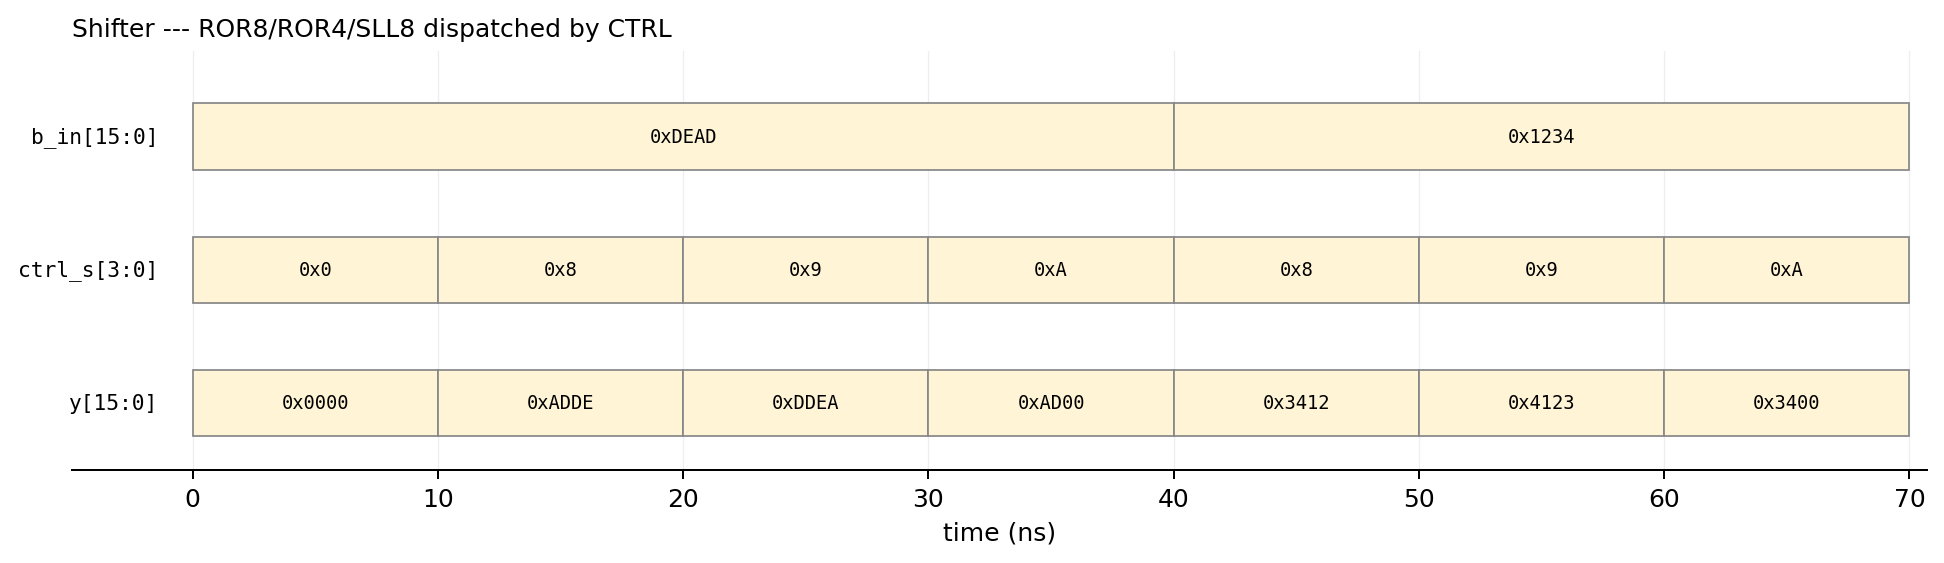
\includegraphics[width=\linewidth]{figures/waveform_shifter.png}
  \caption{Shifter waveform (\texttt{report/vcd/shifter.vcd}).}
  \label{fig:wave-shifter}
\end{figure}

The output column on \texttt{0xDEAD} matches the rule table exactly:
ROR8 ($1000$) $\to$ \texttt{0xADDE}, ROR4 ($1001$) $\to$ \texttt{0xDDEA},
SLL8 ($1010$) $\to$ \texttt{0xAD00}. The undefined opcode \texttt{0x0}
correctly produces \texttt{0x0000}.

\paragraph{ALU.}
Figure~\ref{fig:wave-alu} is the existing
\texttt{tb/alu\_tb.vhdl} sweep across opcodes. The early region
exercises individual opcodes on small operands (with the ALU producing
\texttt{0x0000} for opcodes its body does not decode); the later
region runs through a parameterised vector sweep that ramps
\texttt{ABUS} / \texttt{BBUS} across the address space.

\begin{figure}[H]
  \centering
  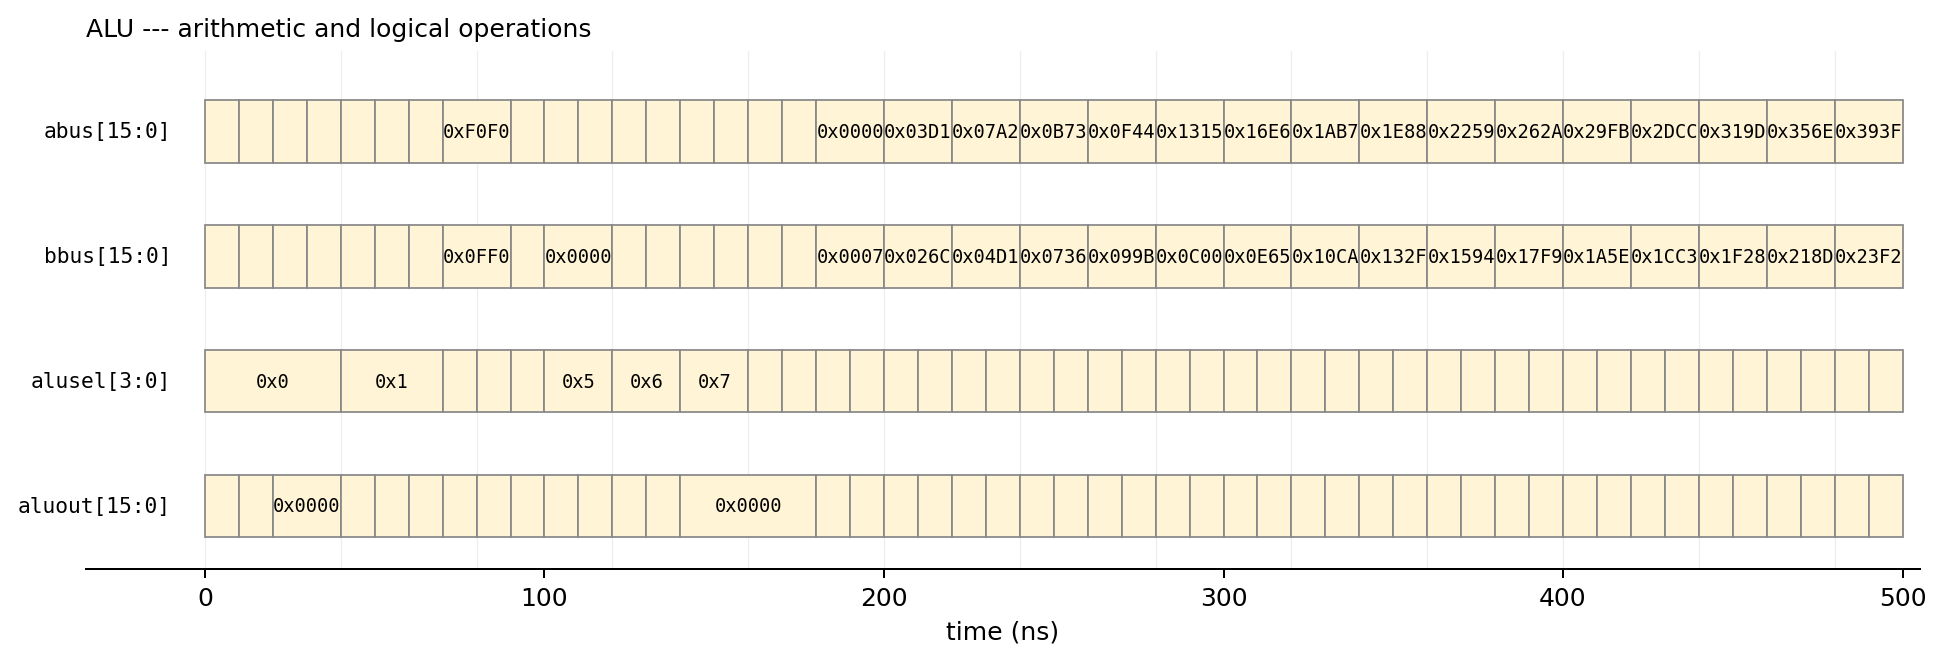
\includegraphics[width=\linewidth]{figures/waveform_alu.png}
  \caption{ALU waveform (\texttt{report/vcd/alu.vcd}).}
  \label{fig:wave-alu}
\end{figure}

\paragraph{Register file.}
Figure~\ref{fig:wave-rf} is the existing
\texttt{waveforms/file\_register\_wave.vcd}.

\begin{figure}[H]
  \centering
  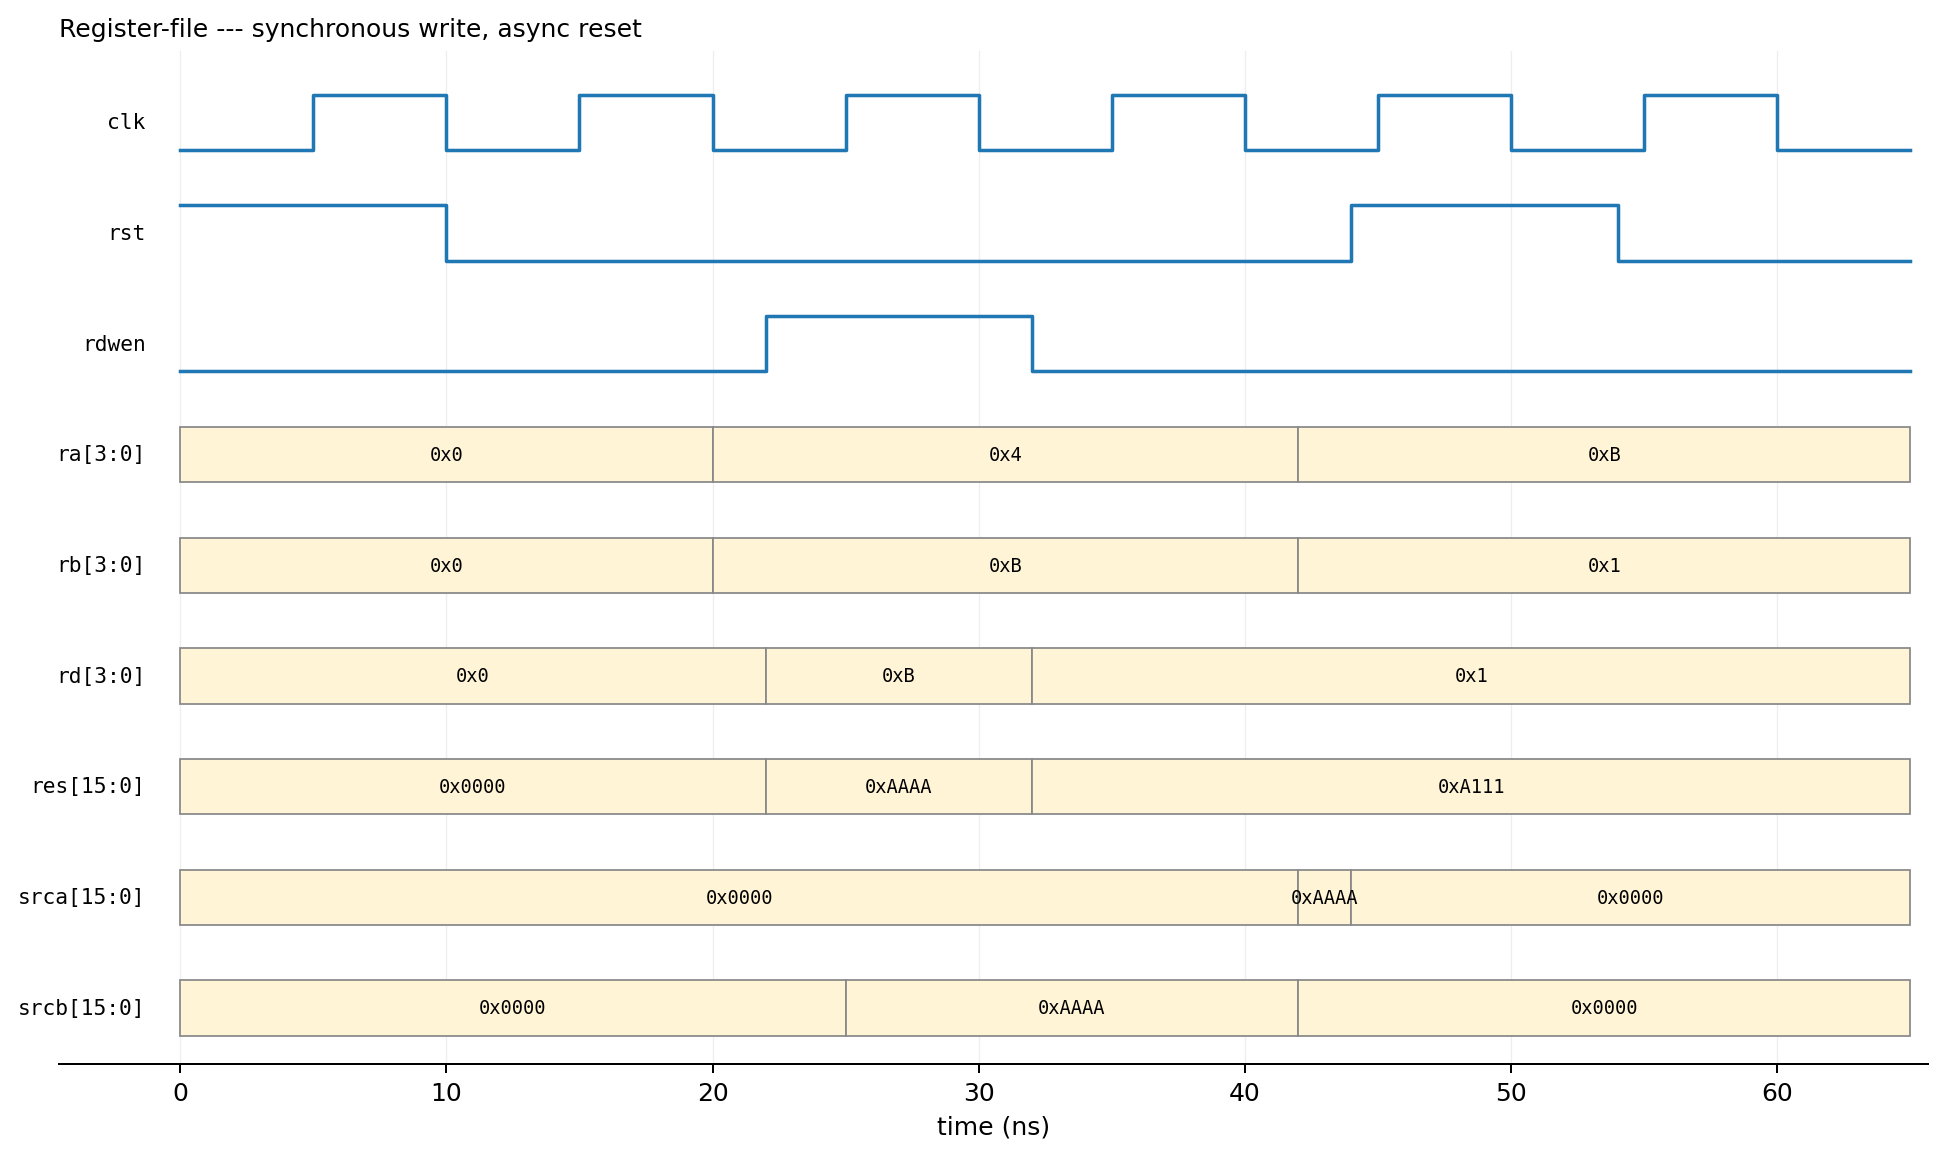
\includegraphics[width=\linewidth]{figures/waveform_register_file.png}
  \caption{Register-file waveform
  (\texttt{waveforms/file\_register\_wave.vcd}).}
  \label{fig:wave-rf}
\end{figure}

Cycle walk-through:
\begin{itemize}[leftmargin=*]
  \item \textbf{0--10\,ns:} \texttt{rst='1'}. Two rising edges occur
        during reset; every entry of the register array is forced to
        \texttt{0x0000}.
  \item \textbf{22\,ns:} \texttt{rdwen} rises with \texttt{rd=0xB},
        \texttt{res=0xAAAA}. On the next rising edge (25\,ns) the
        register file commits \texttt{R[0xB] $\leftarrow$ 0xAAAA};
        \texttt{srcb} (driven by \texttt{rb=0xB}) is observed at
        \texttt{0xAAAA} immediately afterwards.
  \item \textbf{32\,ns:} \texttt{rdwen} is dropped while \texttt{res}
        is changed to \texttt{0xA111}; no write occurs.
  \item \textbf{42\,ns:} read indices switch to \texttt{ra=0xB},
        \texttt{rb=0x1}. \texttt{srca} sees \texttt{0xAAAA} (the
        earlier write); \texttt{srcb} sees \texttt{0x0000}
        (\texttt{R[0x1]} was never written), which is the
        write-enable check.
  \item \textbf{44\,ns:} \texttt{rst} is re-asserted between clock
        edges; \texttt{srca} drops to \texttt{0x0000} immediately,
        confirming the reset is asynchronous.
\end{itemize}

\paragraph{Combinational block.}
Figure~\ref{fig:wave-comb} drives the integrated combinational block
and verifies the CTRL routing.

\begin{figure}[H]
  \centering
  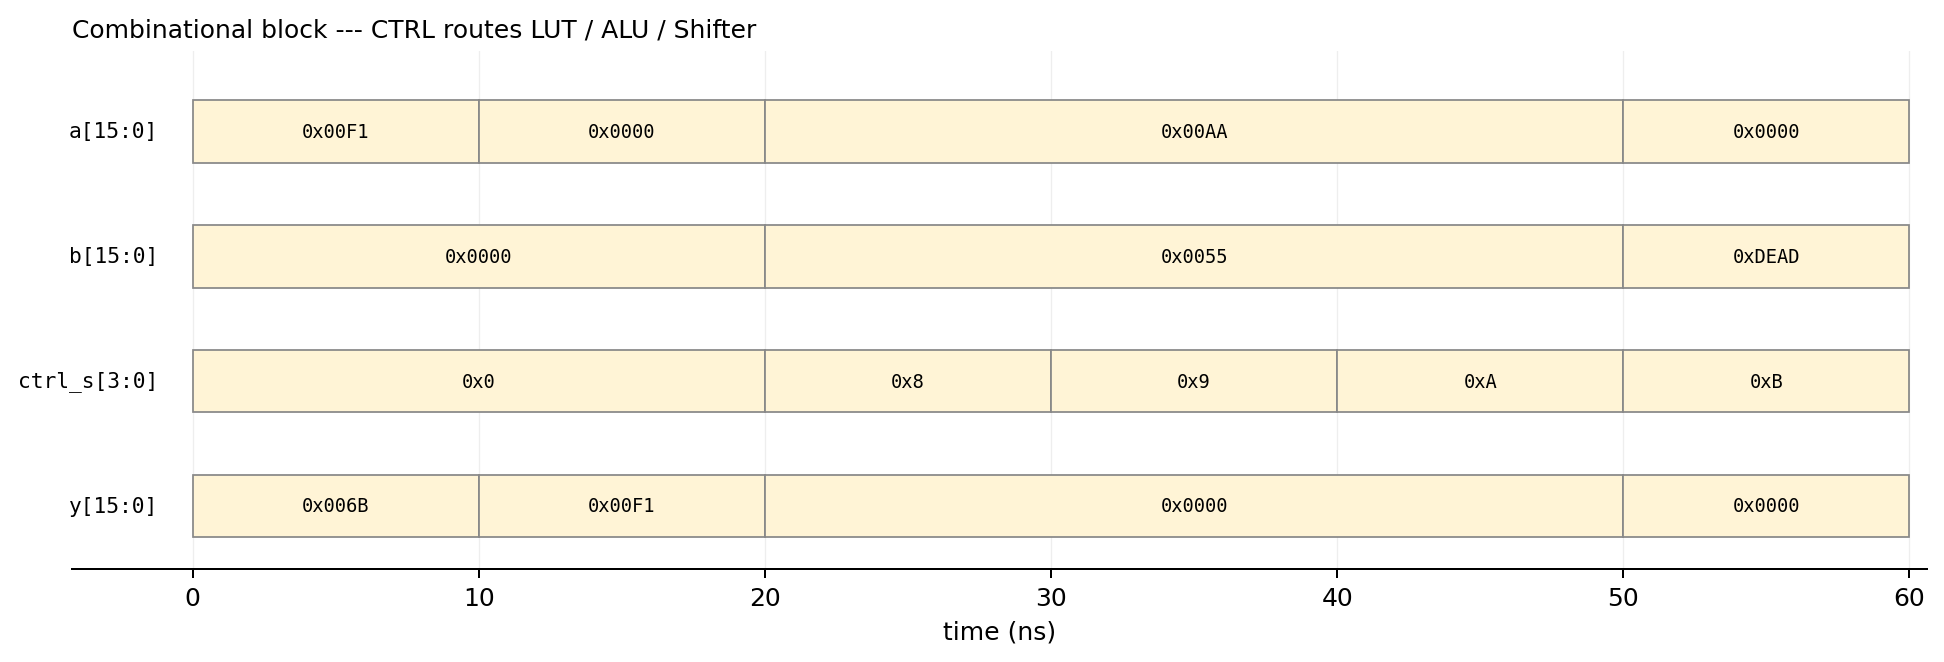
\includegraphics[width=\linewidth]{figures/waveform_combinational_circuit.png}
  \caption{Combinational-block waveform
  (\texttt{report/vcd/combinational\_circuit.vcd}).}
  \label{fig:wave-comb}
\end{figure}

Key transitions:
\texttt{CTRL=0000} with \texttt{A=0x00F1} routes to the LUT and
produces \texttt{0x006B} (the same value the top-level test uses to
verify register write-back);
\texttt{CTRL=0000} with \texttt{A=0x0000} produces the canonical
\texttt{0x00F1};
\texttt{CTRL$\in$\{1000, 1001, 1010\}} routes to the ALU
(\texttt{0x0000} for these undecoded opcodes);
\texttt{CTRL=1011} routes to the shifter, which also returns
\texttt{0x0000} because \texttt{1011} is outside the shifter's
three-opcode table.

\paragraph{Top-level coprocessor.}
Figure~\ref{fig:wave-cop} is the full self-checking
\texttt{coprocessor\_tb} run; the simulator reports
\texttt{All coprocessor tests PASSED} at the end of the trace.

\begin{figure}[H]
  \centering
  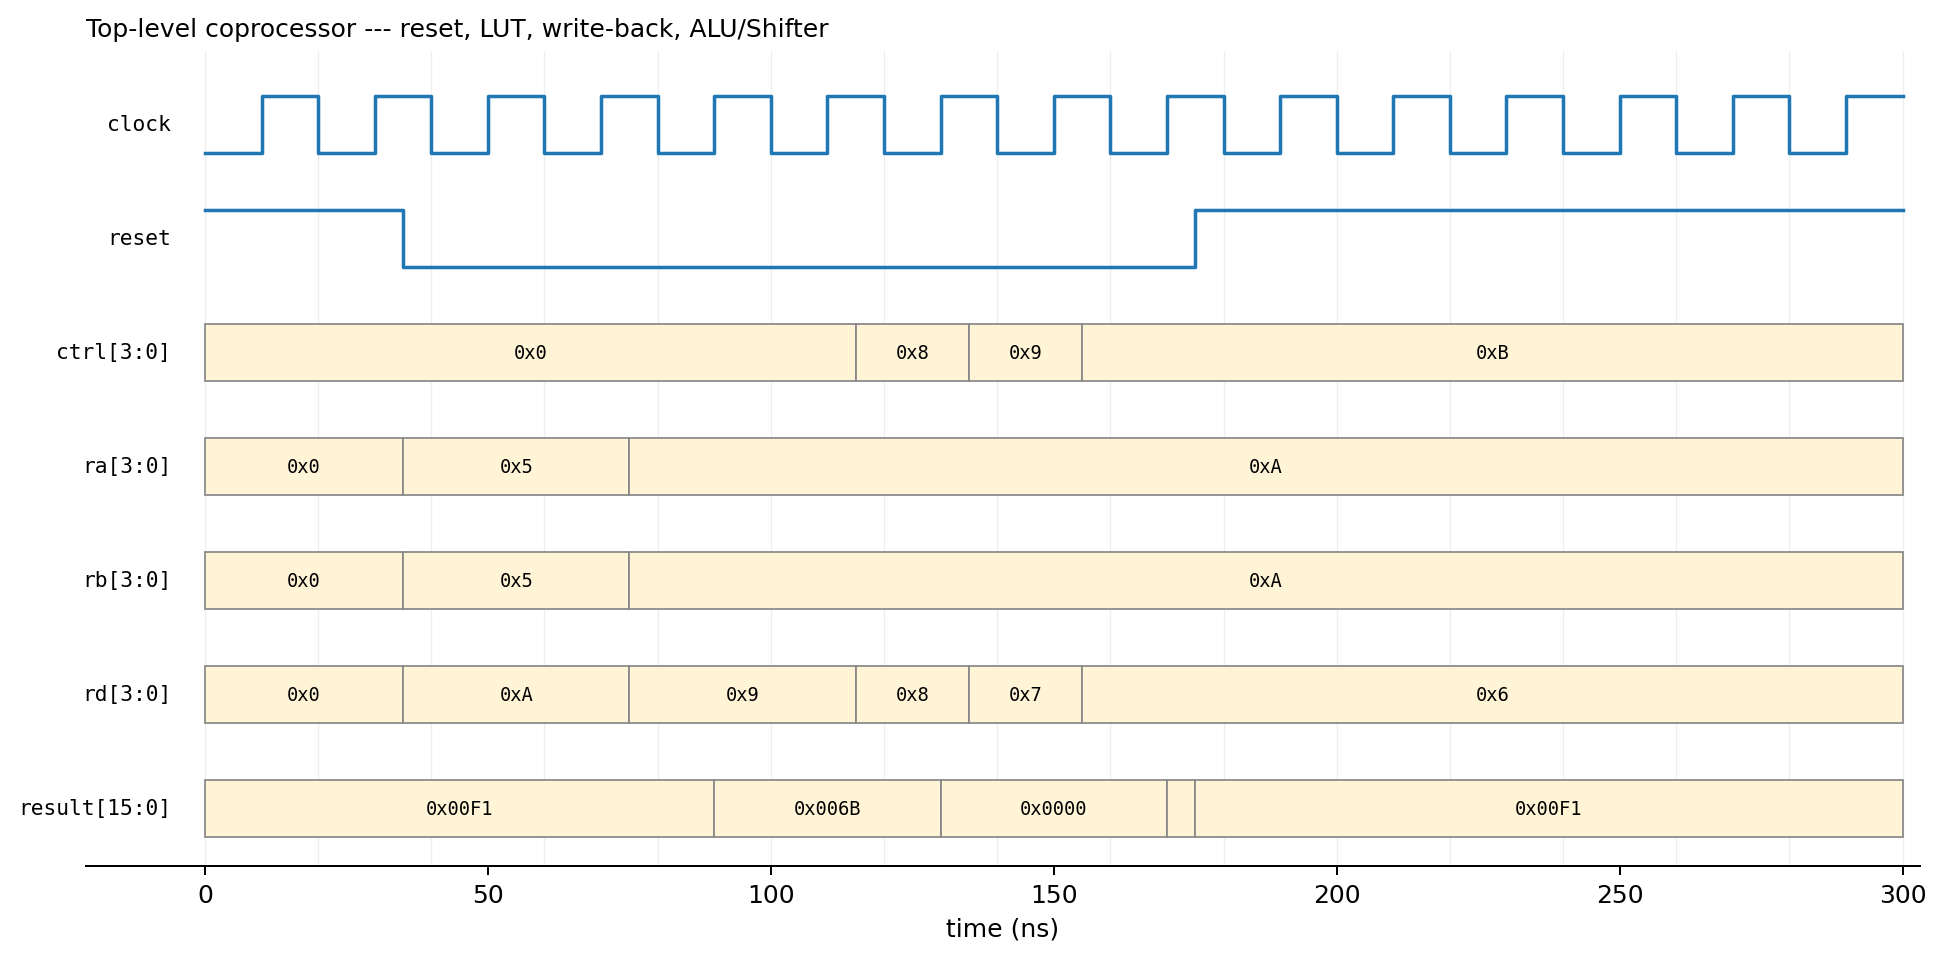
\includegraphics[width=\linewidth]{figures/waveform_coprocessor.png}
  \caption{Top-level coprocessor waveform
  (\texttt{report/vcd/coprocessor.vcd}).}
  \label{fig:wave-cop}
\end{figure}

The five expected \texttt{RESULT} values from
Table~\ref{tab:expected} appear in order: \texttt{0x00F1} during
reset, \texttt{0x00F1} again on the first post-reset LUT read,
\texttt{0x006B} as the write-back probe, then \texttt{0x0000} for
each of the ALU and Shifter steps, and \texttt{0x00F1} once more when
reset is re-asserted.

% =====================================================================
% REFERENCES
% =====================================================================
\newpage
\begin{thebibliography}{9}

\bibitem{sbox-coproc-fpga}
\emph{FPGA-based implementation of an S-Box cryptographic
co-processor for high-performance applications}, ResearchGate, 2025.
The closest published match to this project: a combinational
logic unit that integrates an ALU, a shifter, and a non-linear
S-Box lookup, dispatched by a control unit, targeted at Spartan-6
in VHDL.\\
\url{https://www.researchgate.net/publication/397429210_FPGA-based_implementation_of_an_S-Box_cryptographic_co-processor_for_high-performance_applications}

\bibitem{uthm-coproc}
\emph{Hardware Implementation of a Cryptographic Coprocessor},
UTHM Journal of Electrical and Electronic Engineering, 2021.
Peer-reviewed paper describing a coprocessor with an input
register, 16$\times$16 register file, instruction decoder,
control unit, ALU, and an S-Box-based hashing unit, with a
12-instruction ISA that runs independently from the main
processor.\\
\url{https://publisher.uthm.edu.my/periodicals/index.php/eeee/article/view/4634}

\bibitem{fpga4student}
\emph{Cryptographic Coprocessor Design in VHDL}, fpga4student.com,
2017. Hands-on tutorial with full VHDL for ALU
(ADD/SUB/AND/OR/XOR/NOT/MOV), shifter
(ROR8 = \texttt{1000}, ROR4 = \texttt{1001}, SLL8 = \texttt{1010},
matching this project's encoding), S-Box lookup,
16$\times$16 register file, and the structural top-level.\\
\url{https://www.fpga4student.com/2017/07/cryptographic-coprocessor-design-in-vhdl.html}

\bibitem{gh-sakshi}
S.~Sakshi,
\emph{Cryptographic-coprocessor} (VHDL modules: ALU, register file,
shifter, structural top), GitHub.\\
\url{https://github.com/2331sakshi/Cryptographic-coprocessor}

\bibitem{gh-aidansmyth}
A.~Smyth,
\emph{Cryptographic-Coprocessor} (Xilinx ISE design, synthesis, and
testbench with lookup tables, ALU, and shifter), GitHub.\\
\url{https://github.com/aidansmyth95/Crytpographic-Coprocessor}

\end{thebibliography}

\end{document}
